\section{Experiments}
\label{sec:experiments}

We train a ResNet-18 with the objective of \eqref{eq:loss} on CIFAR-10 for 100 epochs at batch size $512$, with AdamW \citep{loshchilov2017adamw} at learning rate $10^{-3}$ and cosine decay, $\alpha_0 = 0.99$ for the EMA teacher, and $w_\text{sig} = 1$, $\gamma = 10^{-3}$, $\varepsilon = 0.5$ as described in \secref{sec:method}. The projection head output dimension is $d = 256$. Evaluations are performed on the CIFAR-10 validation set using $k$-nearest-neighbour classification with $k = 20$ over $\ell_2$-normalized features; linear-probe accuracies are qualitatively consistent.

Under these settings the model reaches $k$-NN accuracy $77.3\%$ at epoch $100$ (compared to $67.8\%$ for a smaller ConvNet under the same objective; $75.1\%$ on the subset of $10{,}000$ validation images used for geometric analysis below). The absolute number is modest---this is a short training run with only two views and limited augmentation---but the \emph{geometry} of the learned features is what we analyze below.

\subsection{Feature Geometry}
\label{sec:geometry}

We extract the projection-head output for all $10{,}000$ validation images and compute summary statistics of the resulting $10{,}000 \times 256$ matrix $\mat{Z}$.

\paragraph{Per-dimension marginals.} The empirical mean along each dimension is $\mu = -0.008 \pm 0.171$ (mean $\pm$ standard deviation across dimensions) and the variance is $\sigma_j^2 = 0.889 \pm 0.021$---close to unit variance per dimension, with very small spread across dimensions. The mean absolute off-diagonal correlation is $0.013$ with a maximum of $0.069$: dimensions are decorrelated to well within typical significance thresholds.

\paragraph{Norm distribution.} The feature norm distribution has $\E\|\vect{z}\| = 15.21$, $\text{std}\|\vect{z}\| = 1.93$. If the features were exactly $\mathcal{N}(\vect{0}, \mat{I}_{256})$, the norm would follow a $\chi_{256}$ distribution with mean $15.98$ and standard deviation $0.71$. The empirical mean norm matches closely ($95\%$ of the theoretical value), but the empirical standard deviation is roughly three times larger---the distribution is fatter-tailed than a true Gaussian's. This extra radial spread is the signature we study in the rest of this section: it is not an artifact of imperfect training, but a load-bearing degree of freedom the encoder uses.

\subsection{Feature Norm and Prediction Confidence}
\label{sec:norm_confidence}

We divide the validation set into deciles by feature norm and measure $k$-NN accuracy within each decile (\figref{fig:norm_vs_acc}).

\begin{figure}[t]
    \centering
    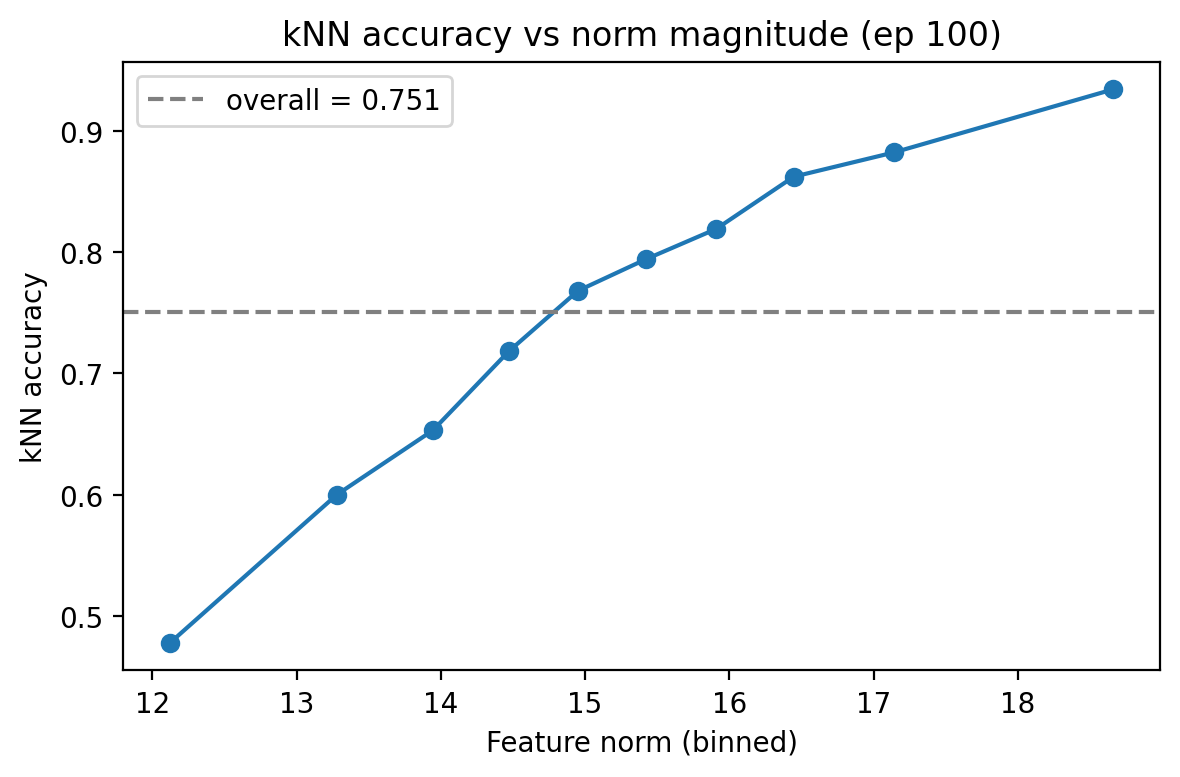
\includegraphics[width=0.52\linewidth]{figures/norm_vs_accuracy_ep100.png}
    \caption{$k$-NN accuracy on CIFAR-10 validation conditioned on feature-norm decile. Accuracy rises from $43.6\%$ in the lowest-norm decile to $91.8\%$ in the highest. Horizontal line: overall accuracy ($73.4\%$ at the epoch shown).}
    \label{fig:norm_vs_acc}
\end{figure}

Accuracy rises monotonically from $43.6\%$ in the lowest-norm decile (features with $\|\vect{z}\| \approx 12$) to $91.8\%$ in the highest (features with $\|\vect{z}\| \approx 19$). Without ever being trained to produce confidence scores, the encoder's feature norm provides a ranking of test samples that is strongly predictive of classification accuracy.

\paragraph{Relation to class structure.} We computed the Pearson correlation between $\|\vect{z}_i\|$ and several candidate explanatory variables (\tabref{tab:correlations}). Distance from the empirical class centroid is almost a perfect predictor of norm ($r = 0.988$): samples far from their class centroid have large norms; samples near the centroid have small norms. $k$-NN correctness has a moderate positive correlation; image-level statistics (mean intensity, contrast, saturation) correlate only weakly.

\begin{table}[t]
    \centering
    \begin{tabular}{lrr}
    \toprule
    \textbf{Quantity} & \textbf{Pearson $r$} & \textbf{$p$} \\
    \midrule
    Distance from class centroid (in feature space) & $+0.990$ & $< 10^{-300}$ \\
    $k$-NN correctness (1/0) & $+0.296$ & $4 \times 10^{-201}$ \\
    Grayscale entropy of input image & $-0.209$ & $5 \times 10^{-99}$ \\
    Raw image mean intensity & $+0.138$ & $8 \times 10^{-44}$ \\
    Raw image standard deviation (contrast) & $+0.050$ & $5 \times 10^{-7}$ \\
    Color saturation & $-0.030$ & $3 \times 10^{-3}$ \\
    \bottomrule
    \end{tabular}
    \caption{Pearson correlation between feature norm and other per-sample quantities, over the $10{,}000$ CIFAR-10 validation images. Negative correlation with image entropy indicates that simpler (lower-entropy) images get higher norms.}
    \label{tab:correlations}
\end{table}

Taken together, these suggest an interpretation: the encoder places ``canonical'' samples of each class far from the origin and ``atypical'' samples near the origin. Atypical samples are also, unsurprisingly, harder to classify correctly, which is why norm and $k$-NN correctness are correlated.

\subsection{Embeddings Under Noise Corruption}
\label{sec:noise}

To probe the confidence hypothesis directly, we linearly interpolate each input with a fixed sample of uniform random noise:
\begin{equation}
    \tilde{x}(\alpha) = (1 - \alpha) x + \alpha \xi, \qquad \xi \sim \text{Unif}[0, 1]^{3 \times 32 \times 32},
\end{equation}
and compute $\|\vect{z}(\alpha)\| = \|f_\theta(\tilde{x}(\alpha))\|$ for $\alpha \in \{0, 0.1, \dots, 1\}$ on $100$ samples (ten per class). \figref{fig:noise_summary} summarizes the response.

\begin{figure}[t]
    \centering
    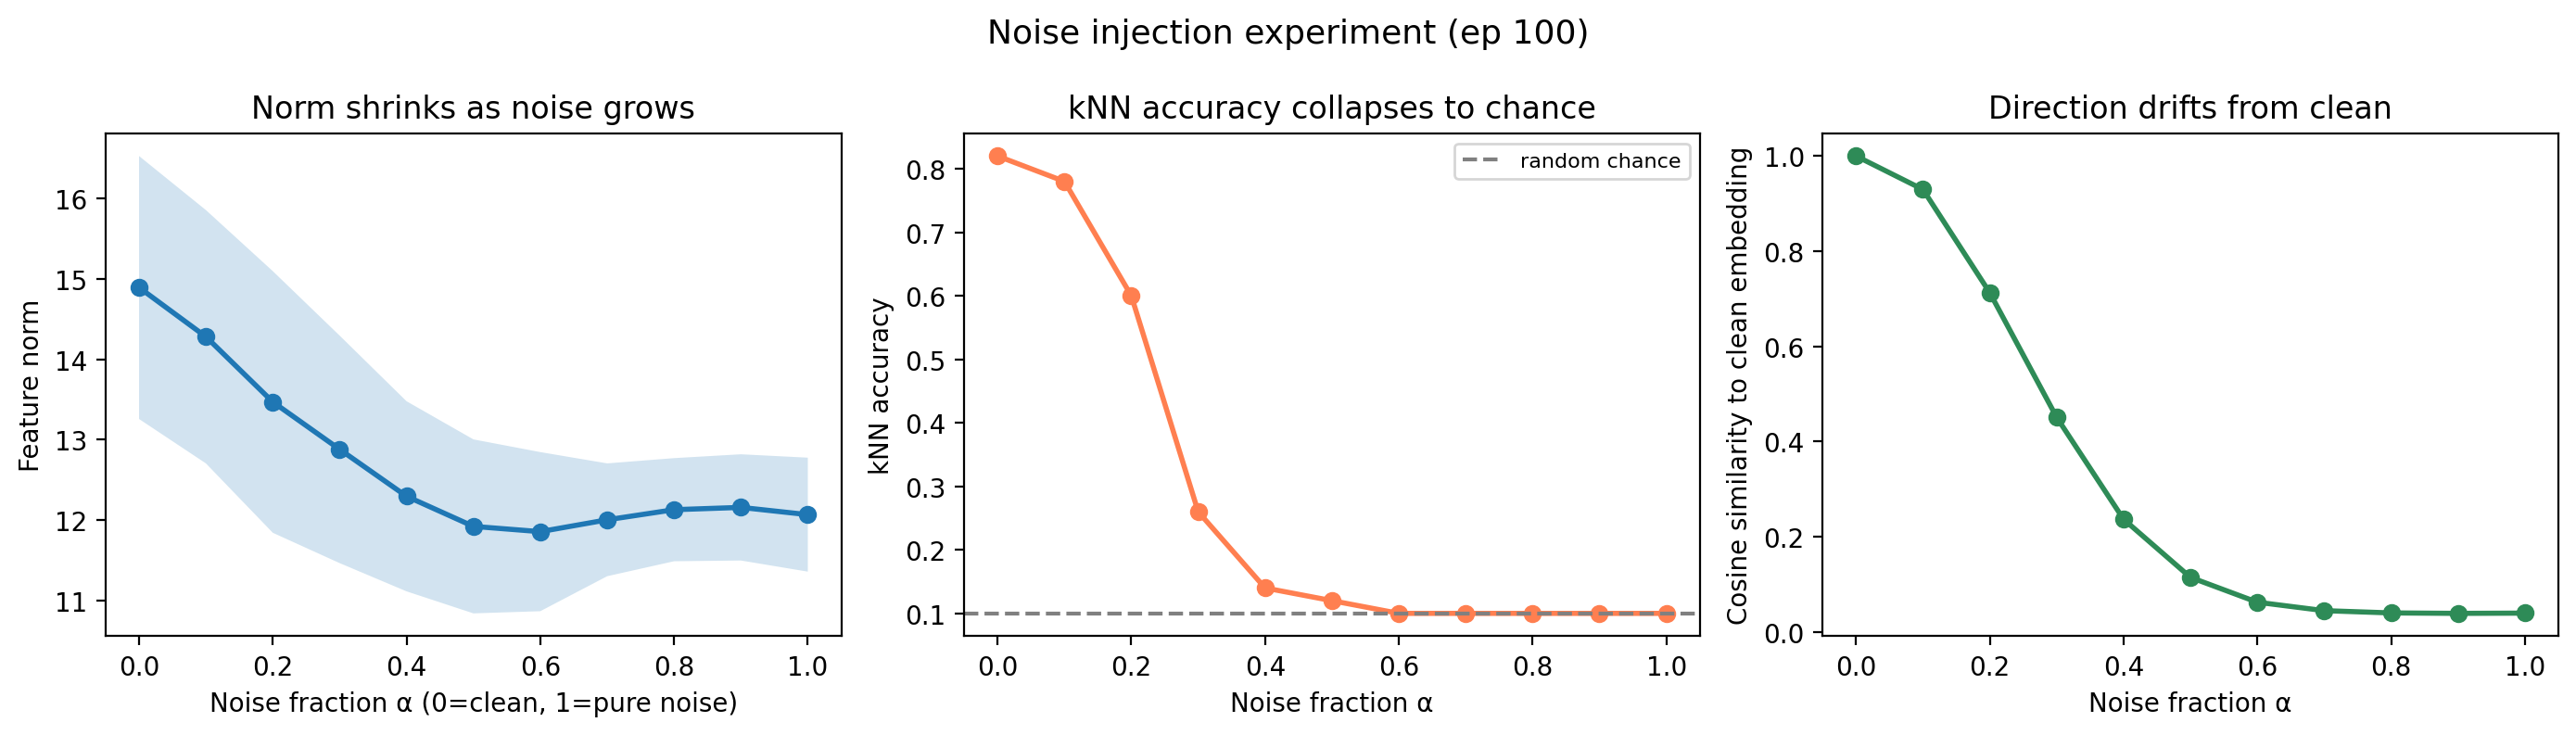
\includegraphics[width=\linewidth]{figures/noise_summary_ep100.png}
    \caption{Noise-mixing response of the flat-Gaussian SSL encoder. Left: feature norm decreases from $14.8$ at $\alpha = 0$ to a floor of $\sim 11.5$ at $\alpha \approx 0.5$, with a slight uptick back to $\sim 12$ at pure noise. Middle: $k$-NN accuracy collapses to chance by $\alpha \approx 0.5$. Right: cosine similarity to the clean embedding decays smoothly. Shaded regions are per-sample standard deviations.}
    \label{fig:noise_summary}
\end{figure}

Mean feature norm drops from $14.89$ at $\alpha = 0$ to $11.92$ at $\alpha = 0.5$ and plateaus near $11.9$--$12.2$ for $\alpha \ge 0.5$, with a small \emph{increase} from $\alpha = 0.6$ to $\alpha = 1.0$ discussed below. Simultaneously, $k$-NN accuracy on this subset collapses from $82\%$ at $\alpha = 0$ to $12\%$ (approaching chance) by $\alpha = 0.5$ (note: the clean accuracy is on a $100$-sample stratified subset; the full-validation-set clean accuracy is $75\%$). The cosine similarity between the noisy and clean embeddings decays smoothly from $1$ to near zero, indicating that the direction of the feature also drifts, but more gradually than the norm collapses.

\paragraph{A stable ``noise manifold''.} The fact that the feature norm does not continue to fall as $\alpha \to 1$---and in fact rises slightly---is notable. Different noise samples all produce features of similar norm $\sim 12.1$, suggesting that pure-noise inputs are mapped to a consistent region of embedding space rather than to arbitrary locations. We characterize this region directly in \secref{sec:noise_subspace}.

\subsection{The Noise Subspace}
\label{sec:noise_subspace}

We embed $2{,}000$ real CIFAR-10 validation images and $500$ independent pure-noise images through the same encoder, and compare the two feature sets.

\paragraph{Effective dimensionality.} We measure effective dimensionality as $\exp\!\left(-\sum_i p_i \log p_i\right)$, where $p_i$ is the $i$-th entry of the normalized PCA spectrum. For the real-image features this is $\approx 237$ of $256$; for noise features it is $\approx 12$. Pure noise collapses into roughly $5\%$ of the ambient dimensionality (\figref{fig:noise_subspace_pca}, top).

\paragraph{Angular relationship to classes.} Let $\bar{\vect{z}}_c$ denote the mean feature of class $c$ in the real-image set and $\bar{\vect{z}}_\text{noise}$ the mean noise feature. The angle between $\bar{\vect{z}}_\text{noise}$ and each class mean ranges from $66^\circ$ (\texttt{frog}) to $82^\circ$ (\texttt{ship}); the mean angle between distinct class means is $63^\circ$. Noise is, in angular terms, \emph{further} from every class than classes are from each other---it occupies a direction that is roughly orthogonal to the class manifold.

\paragraph{UMAP.} \figref{fig:noise_subspace_pca} (bottom) shows a UMAP \citep{mcinnes2018umap} embedding of the real-image and noise features. The two sets are completely disjoint in the projection: noise forms a tight cluster that does not overlap any class region.

\begin{figure}[t]
    \centering
    \begin{subfigure}{\linewidth}
        \centering
        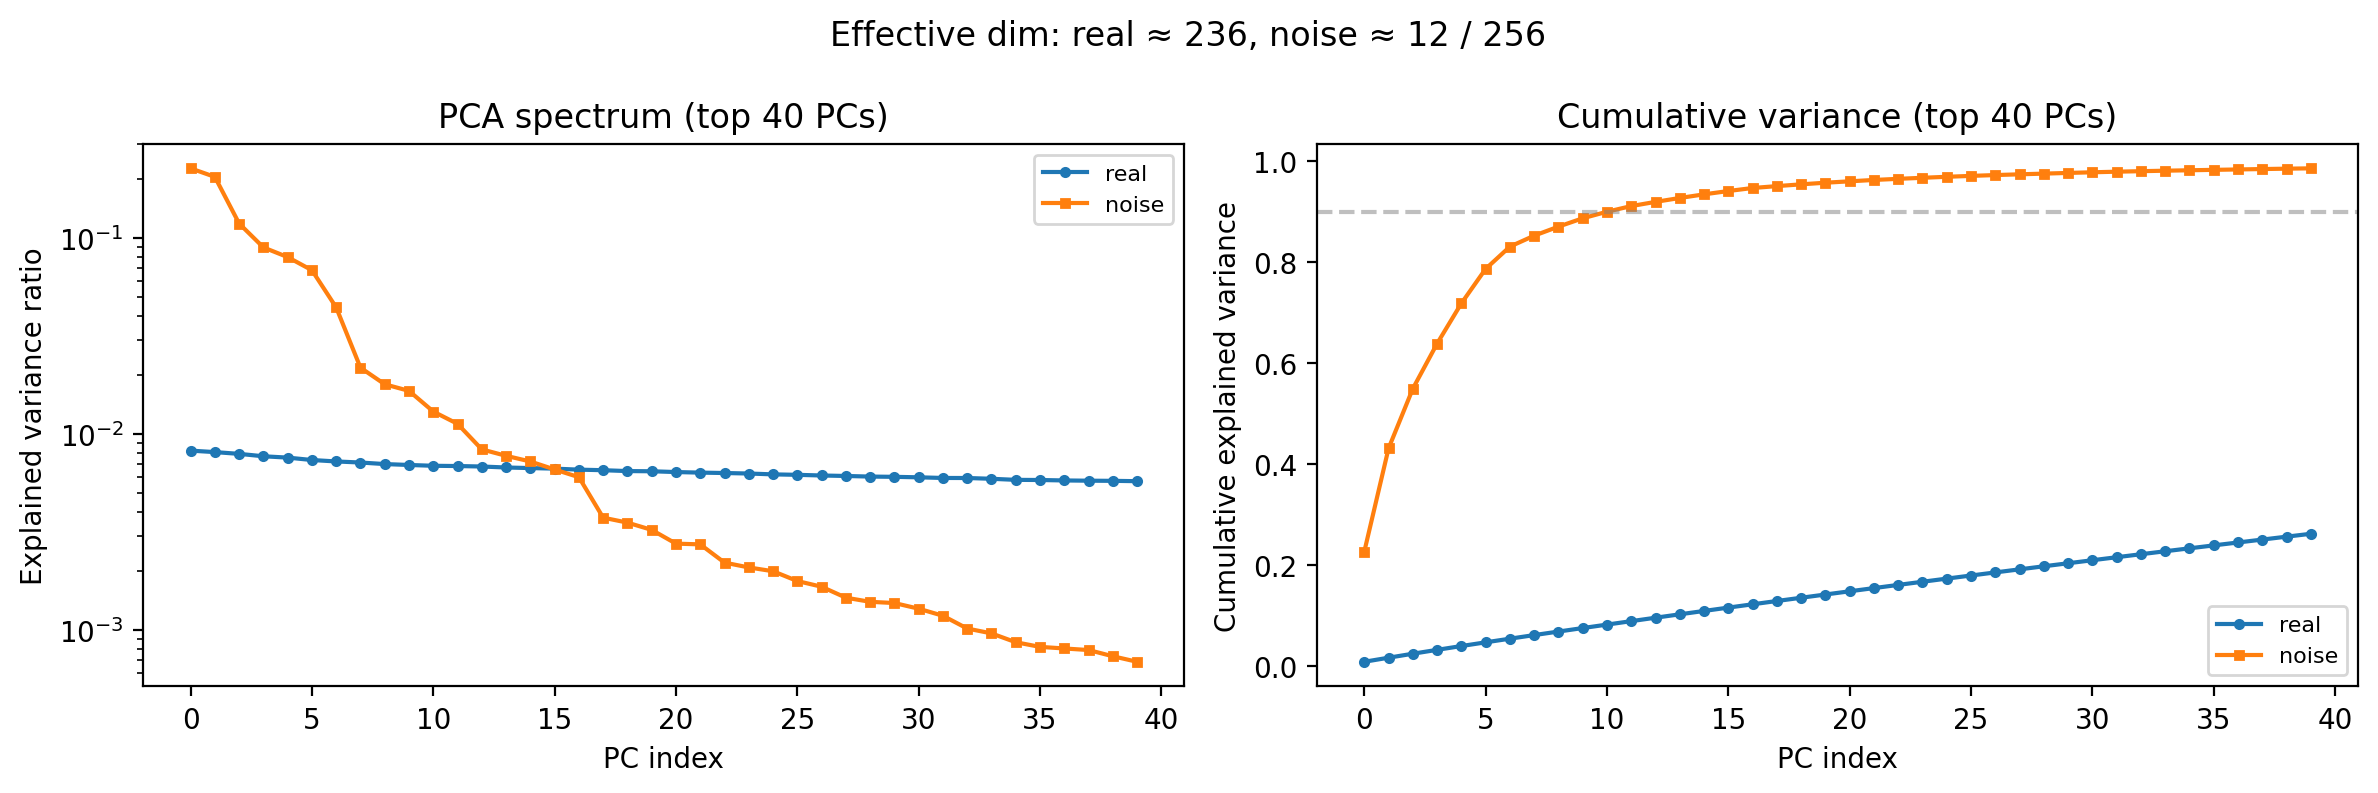
\includegraphics[width=0.9\linewidth]{figures/noise_subspace_pca_ep100.png}
    \end{subfigure}\\[3pt]
    \begin{subfigure}{\linewidth}
        \centering
        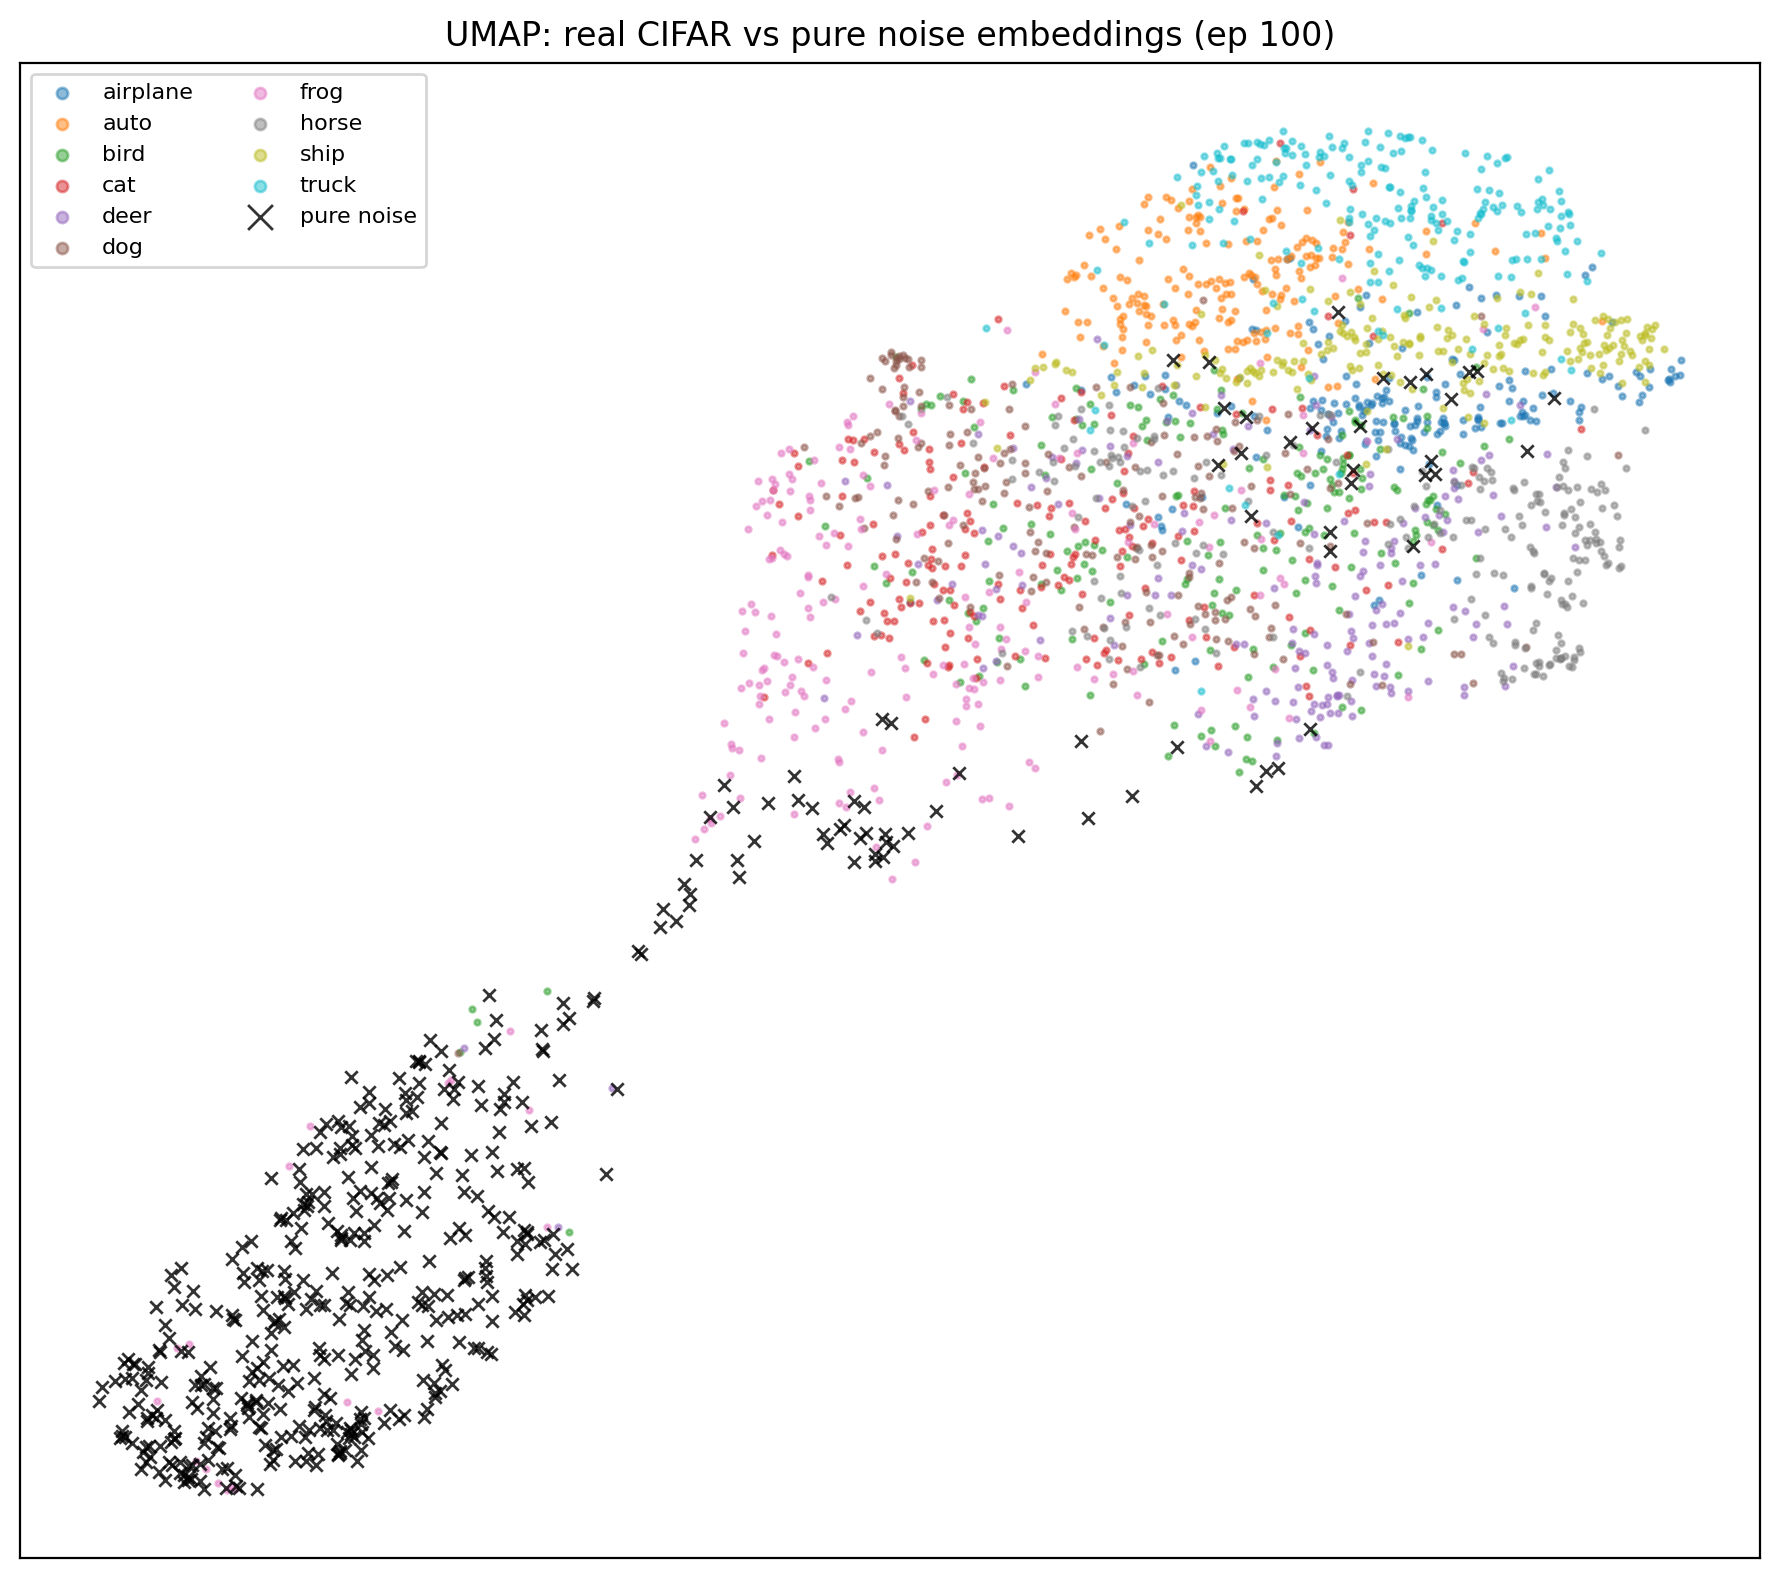
\includegraphics[width=0.55\linewidth]{figures/noise_subspace_umap_ep100.png}
    \end{subfigure}
    \caption{Top: PCA spectrum of real (flat) vs noise (steep) features; effective dimensions are $237$ and $12$ respectively. Bottom: UMAP embedding of the combined feature set. Noise samples ($\times$) form a cluster completely disjoint from the real-image classes.}
    \label{fig:noise_subspace_pca}
\end{figure}

\subsection{Comparison with DINOv2}
\label{sec:dinov2}

The behaviour documented above could be a generic property of joint-embedding SSL, or it could be specific to the flat-Gaussian geometry. To distinguish these, we repeat the noise-mixing experiment on a pretrained DINOv2 ViT-S/14 model \citep{oquab2023dinov2}, using the (unnormalized) CLS token and the mean-pooled patch tokens from \texttt{forward\_features}. CIFAR-10 inputs are bilinearly upsampled from $32 \times 32$ to $224 \times 224$ to match DINOv2's expected resolution. The same noise-mixing protocol applies.

\begin{figure}[t]
    \centering
    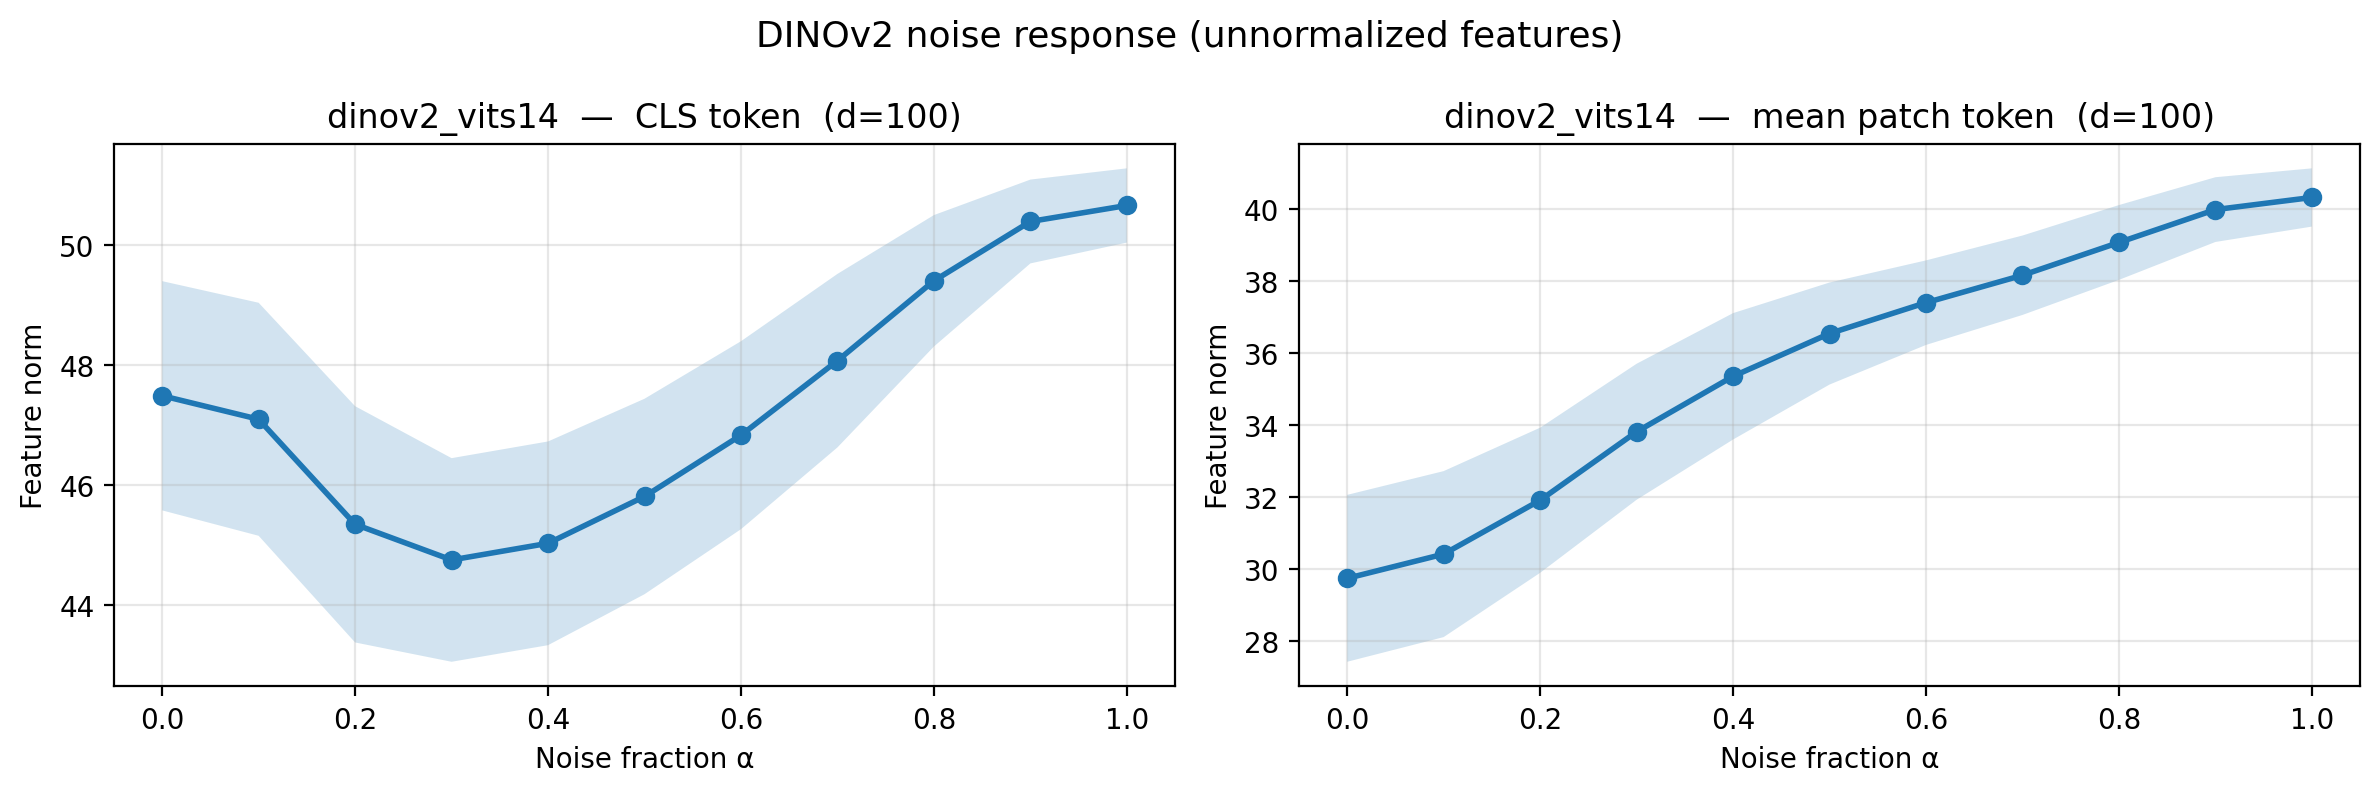
\includegraphics[width=\linewidth]{figures/noise_dinov2_dinov2_vits14.png}
    \caption{DINOv2 ViT-S/14 noise response. Left: CLS token norm has a shallow dip at $\alpha \approx 0.3$ and then \emph{rises} past the clean value, reaching a maximum at $\alpha = 1$. Right: mean-pooled patch-token norm rises \emph{monotonically} with noise fraction. In contrast to \figref{fig:noise_summary}, pure noise produces the highest-norm features.}
    \label{fig:noise_dinov2}
\end{figure}

\figref{fig:noise_dinov2} shows the result. Both of DINOv2's backbone features behave very differently from our flat-space features:
\begin{itemize}
    \item The CLS-token norm has a shallow V-shape, dipping from $47.5$ (clean) to $44.8$ at $\alpha = 0.3$, then \emph{rising} back above clean to $50.7$ at pure noise. There is no monotone relationship between noise fraction and feature norm.
    \item The mean patch-token norm rises \emph{monotonically} with noise from $29.8$ (clean) to $40.3$ (pure noise). Higher norm corresponds to \emph{lower} confidence.
\end{itemize}

Whatever mechanism causes noise inputs in our flat-Gaussian model to migrate toward the origin and occupy a low-dimensional subspace is not a generic property of self-supervised ViTs. DINOv2, trained with a cross-entropy-over-prototypes objective on normalized features, does not learn such a structure; if anything, its feature norm anti-correlates with confidence.

\paragraph{Caveat.} CIFAR inputs upsampled to $224 \times 224$ are mildly out-of-distribution for DINOv2 (trained on ImageNet at native resolution). The pattern warrants re-testing on native ImageNet validation images; preliminary runs (not shown) show the same qualitative direction, but a more careful comparison is future work.

\subsection{Summary of Findings}

We have shown, for a ResNet-18 trained on CIFAR-10 with a minimal flat-Gaussian SSL objective:
\begin{enumerate}
    \item the feature norm is strongly correlated with $k$-NN accuracy, with high-norm samples classified at $\approx 2\times$ the accuracy of low-norm samples;
    \item the norm is almost perfectly correlated ($r = 0.99$) with distance from the class centroid in feature space;
    \item adding uniform noise to the input radially contracts the embedding toward a stable low-norm region;
    \item pure-noise inputs collapse into a $\sim 13$-dimensional subspace, oriented roughly orthogonal to every class direction;
    \item none of the above is present in the publicly available DINOv2 model; if anything, the sign of the relationship is reversed.
\end{enumerate}

The combination suggests that feature norm in flat-Gaussian SSL encodes something close to a confidence or canonicalness score, without any supervised signal to that effect. We discuss interpretation and limitations in the next section.
